% use the answers clause to get answers to print; otherwise leave it out.
\documentclass[11pt,addpoints,answers]{exam}
%\documentclass[11pt,addpoints]{exam}
\RequirePackage{amssymb, amsfonts, amsmath, latexsym, verbatim, xspace, 
setspace, wasysym}
\usepackage{graphicx}

% By default LaTeX uses large margins.  This doesn't work well on exams; problems
% end up in the "middle" of the page, reducing the amount of space for students
% to work on them.
\usepackage[margin=1in]{geometry}
\usepackage{enumerate}
\usepackage[hidelinks]{hyperref}
\usepackage{subfig}

% Here's where you edit the Class, Exam, Date, etc.
\newcommand{\class}{NPRE 560}
\newcommand{\term}{Fall 2024}
\newcommand{\assignment}{HW 3}
\newcommand{\duedate}{2024.10.23}
%\newcommand{\timelimit}{50 Minutes}
\newcommand{\StudentName}{Oleksandr Yardas} %Please include your name here

\newcommand{\nth}{n\ensuremath{^{\text{th}}} }
\newcommand{\ve}[1]{\ensuremath{\mathbf{#1}}}
\newcommand{\Macro}{\ensuremath{\Sigma}}
\newcommand{\vOmega}{\ensuremath{\hat{\Omega}}}

% For an exam, single spacing is most appropriate
\singlespacing
% \onehalfspacing
% \doublespacing

% For an exam, we generally want to turn off paragraph indentation
\parindent 0ex

%\unframedsolutions

\begin{document} 
This homework was done in collaboration with Luke Seifert and Anthony Boyd

% These commands set up the running header on the top of the exam pages
\pagestyle{head}
\firstpageheader{}{}{}
\runningheader{\class}{\assignment\ - Page \thepage\ of \numpages}{Due \duedate}
\runningheadrule

\class \hfill \StudentName \hfill \term \\
\assignment \hfill Due \duedate\\
\rule[1ex]{\textwidth}{.1pt}
%\hrulefill

%%%%%%%%%%%%%%%%%%%%%%%%%%%%%%%%%%%%%%%%%%%%%%%%%%%%%%%%%%%%%%%%%%%%%%%%%%%%%%%%%%%%%
%%%%%%%%%%%%%%%%%%%%%%%%%%%%%%%%%%%%%%%%%%%%%%%%%%%%%%%%%%%%%%%%%%%%%%%%%%%%%%%%%%%%%
\begin{itemize}
        \item Show your work. 
        \item This work must be submitted online as a \texttt{.pdf} through Canvas.
        \item Work completed with LaTeX or Jupyter earns 1 extra point. Submit 
                source file (e.g. \texttt{.tex} or \texttt{.ipynb}) along with 
                the \texttt{.pdf} file.
        \item If this work is completed with the aid of a numerical program 
                (such as Python, Wolfram Alpha, or MATLAB) all scripts and data 
                must be submitted in addition to the \texttt{.pdf}.
        \item If you work with anyone else, document what you worked on together.
\end{itemize}
\rule[1ex]{\textwidth}{.1pt}

% ---------------------------------------------
\begin{questions}
        \question (Ott Review 6.20) Describe in words, with graphs, and with 
        formulas the transient following a step change in reactivity or source:
        \begin{parts}
                \part[5] Without delayed neutrons.
                \begin{solution}
                    With no delayed neutrons, we drop delayed neutrons from the
                    kinetics equation:
                    \begin{equation}
                        \dot{p} = \frac{\rho(t)}{\Lambda}p(t)
                    \end{equation}
                    Following a step reactivity insertion, the slope of the
                    power will constantly increase at a rate of
                    $\frac{\rho}{\Lambda}\rho$, that is, without any delayed
                    neutrons the power blows up. We can also see this if we
                    solve the equation analytically, assuming the reactivity
                    stays constant, as $p(t) = p_{0} e^{\frac{\rho}{\Lambda}t}$.
                    Figure \ref{fig:1a} shows a plot of the power over time
                    using $p_{0} = 1.0$, $\Lambda = 2 \cdot 10^{-5}$. The below
                    figure shows a plot of the reactivity insertion without
                    delayed neutrons.
                    \begin{center}
                        \centering
                        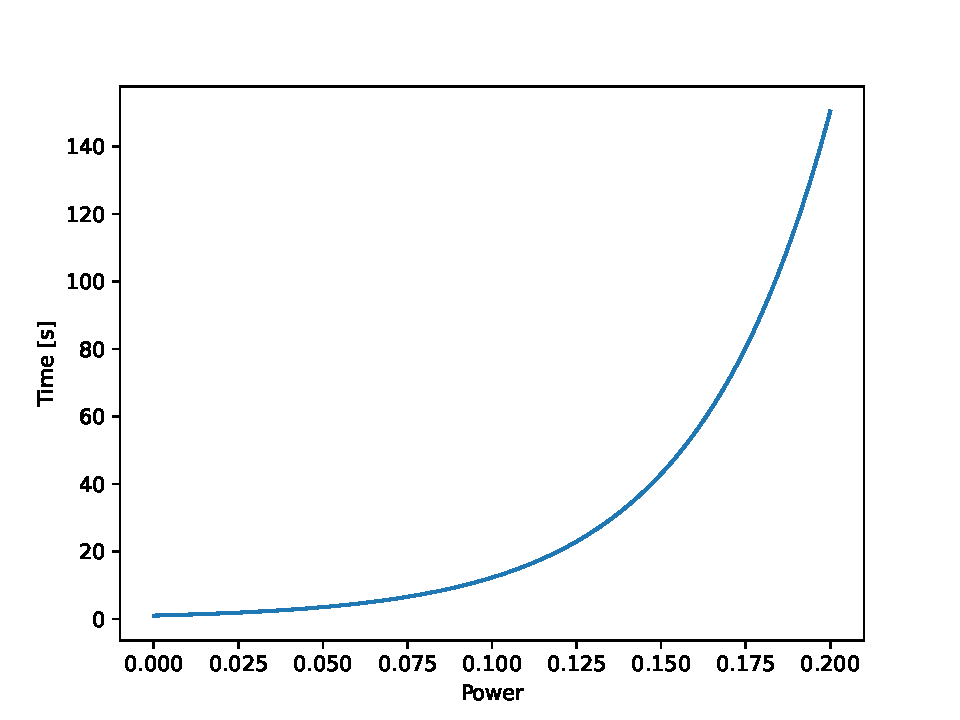
\includegraphics[width=0.5\linewidth]{1a.pdf}
                        %\caption{Plot of reactivity insertion without delayed
                        %neutrons}
                        \label{fig:1a}
                    \end{center}
                \end{solution}

                \part[5] With constant delayed neutron source.
                \begin{solution}
                    With a constant delayed source, we approximate the delayed
                    neutron source as constant, that is $S_d(t) = S_{d} =
                    \beta p_{0}$. Assumuing no external source, the kinetics
                    equation becomes
                    \begin{equation}
                        \dot{p} = \frac{\rho(t) - \beta}{\Lambda}p(t) +
                        \frac{\beta p_{0}}{\Lambda}
                    \end{equation}
                    The transient following a step reactivity insertion depends
                    on the value of $\beta$. If $\beta \gg \rho$, we will have
                    an inital jump in reactivity that quickly stabilizes. As
                    $\beta > \rho$, the transient takes longer to stabilize. If
                    $\beta = \rho$, the $p(t)$ term dissappaer and we have
                    linear transient. As $\beta$ becomes less than $\rho$, the
                    transient blows up more quickly. The figures below,
                    left-to-right top-to-bottom, show th transient for $\beta$
                    750, 100, 50, and 20 pcm
                        \subfloat{
                            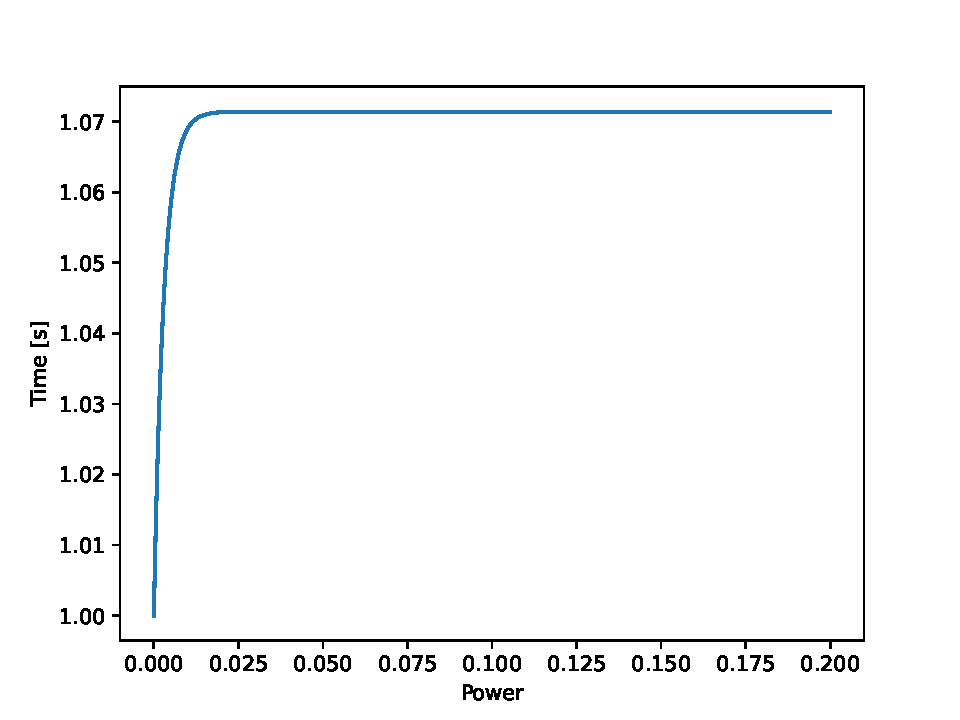
\includegraphics[width=0.5\linewidth]{1b1.pdf}
                            %\label{fig:1b1}
                        }
                        \subfloat{
                            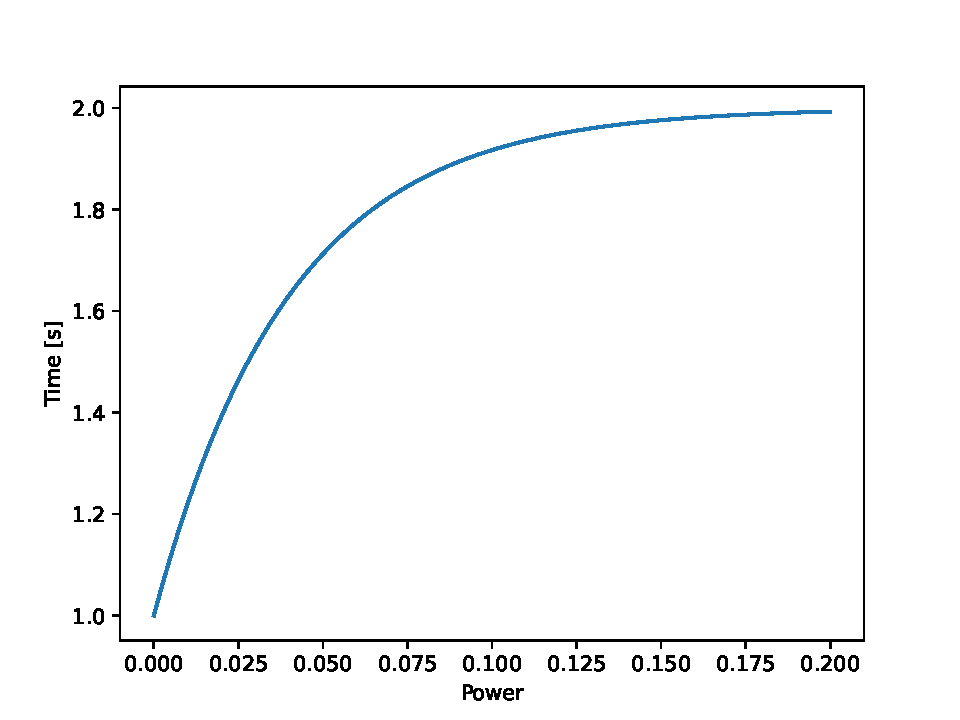
\includegraphics[width=0.5\linewidth]{1b2.pdf}
                            %\label{fig:1b2}
                        }\\
                        \subfloat{
                            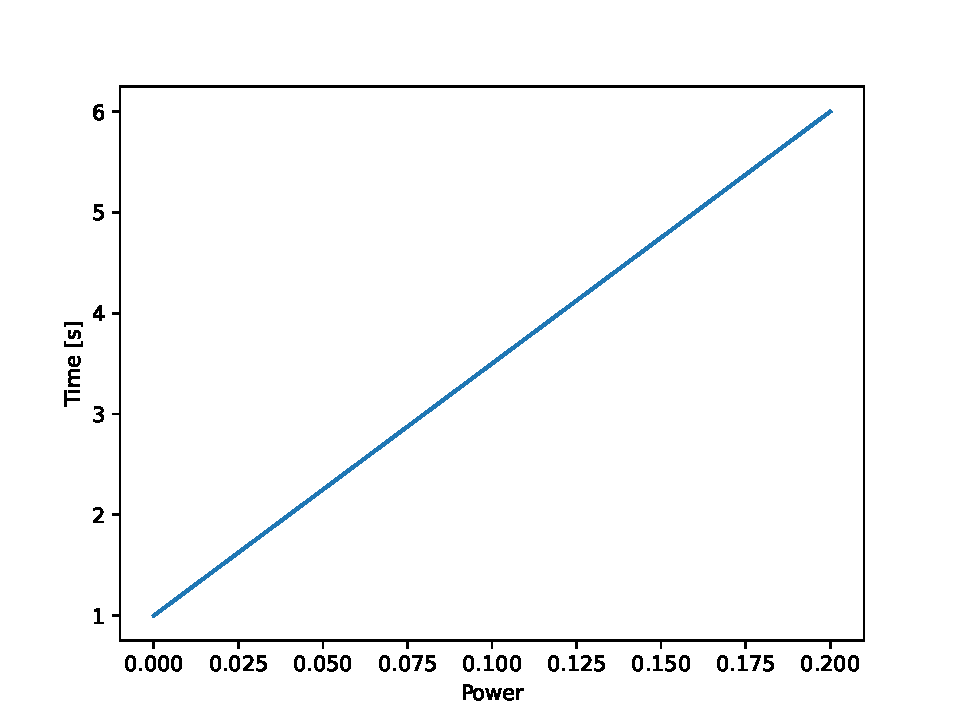
\includegraphics[width=0.5\linewidth]{1b3.pdf}
                            %\label{fig:1b3}
                        }
                        \subfloat{
                            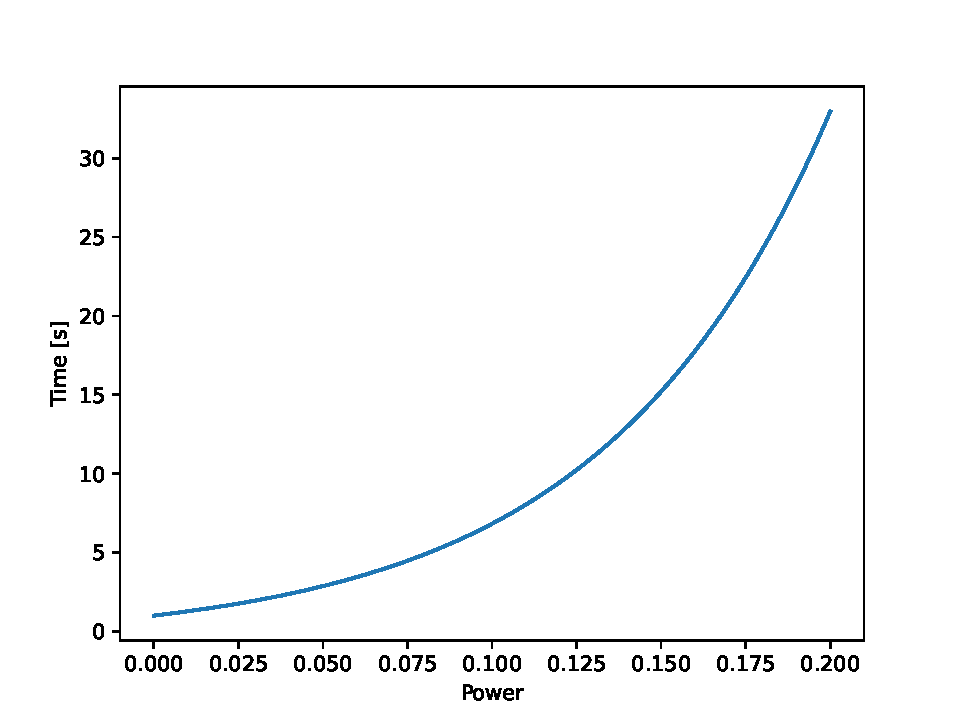
\includegraphics[width=0.5\linewidth]{1b4.pdf}
                            %\label{fig:1b4}
                        }
                        %\caption{Transients for CDS approximation, $P_0 = 1$,
                        %    $\Lambda = 2\cdot 10^{-5}$:
                        %\subref{fig:1b1} Transient when $\beta = 750$ pcm;
                        %\subref{fig:1b2} Transient when $\beta = 100$ pcm;
                        %\subref{fig:1b3} Transient when $\beta = 50$ pcm;
                        %\subref{fig:1b4} Transient when $\beta = 20$ pcm}
                        %\label{fig:cr_eject_results}
                \end{solution}

                \part[5] With no approximations (no formula required).
                \begin{solution}
                    The behavior of the transient in this case will be very
                    similar to the CDS approximation, however this time we have
                    a time-varying delayed neutron source. This is what we
                    studied in CP 1.
                \end{solution}

        \end{parts}

        % ---------------------------------------------
        \question (Ott Review 6.34) Estimate the time it takes to establish the 
        stable asymptotic transient for $\rho_1 < \beta$ in an initially 
        critical reactor.
                \begin{solution}
                    For a critical reactor with a step reactivity instertion to
                    a stationary state $\rho_{1}$ from a stationary state
                    $\rho_{0}$, the response in the power is also a prompt jump.
                    So there will be a transtion to a higer flat power
                    profile corresponding to the prompt jump in reactivity. We
                    can find the time it takes to make this transition based on
                    Equation 6.94 in Ott, the equation or the power when the
                    inverse prompt period is constant (which we have when we are
                    critical):
                    \begin{equation}
                        p(t) = p_0 e^{\alpha_{p} t} + p_0 \frac{\beta}{\beta -
                        \rho_1} (1 - e^{\alpha_{p} t})
                    \end{equation}
                    We have a stable asymptotic transient when $\frac{dp}{dt} =
                    0$:
                    \begin{align*}
                        \frac{dp}{dt} = p_0 \alpha_p e^{\alpha_p t} - p_0 \frac{\beta}{\beta -
                        \rho_1} \alpha_{p} e^{\alpha_{p} t}
                    \end{align*}
                    Setting this equal to zero and rearranging terms yields
                    \begin{equation}
                        0 = p_0 \alpha_p \left(1 - \frac{\beta}{\beta -
                            \rho_1} \right) e^{\alpha_{p} t}
                    \end{equation}
                    If we try to take the log of both sides, we have $\log(0)$
                    which is nonphysical. So if we instead set the LHS equal to
                    some small value $\delta$, we can take the lograithm:
                    \begin{equation}
                        \log(\frac{\delta}{p_0 \alpha_{p} \left(1 -
                        \frac{\beta}{\beta - \rho_1}\right)}) = \alpha t
                    \end{equation}
                    As $\delta$ approaches zero, the LHS blows up towards
                    $-\infty$. I am not sure how to proceed from here :/
                \end{solution}


        % ---------------------------------------------
        \question[10] (Ott Review 6.35) Explain in terms of roots of the 
        characteristic equation:
        \begin{parts}
                \part[5] the prompt jump phenomenon
                \begin{solution}
                    $\lambda_7$ is the smallest root so governs short
                    time-behavior, and is reponsible for the inital dynamics of
                    a prompt jump phenomenon.
                \end{solution}
                \part[5] the delayed neutron induced transition
                \begin{solution}
                    The delayed neutron transition is goverened by the
                    intermediate roots $\lambda_{i}$ for $i=2,3,4,5,6$.
                \end{solution}
                \part[5] the stable period 
                \begin{solution}
                    The stable period is govered by the largest root (i.e. the
                    root yielding the longest period), $\lambda_{1}$
                \end{solution}
        \end{parts}

        
        % ---------------------------------------------
        \question[30] (Ott Problem 10.1) Find the numerical value of $p^{00}$, 
        the flux after a prompt jump for which the increase due to delayed 
        neutrons is just compensated by Doppler feedback, for an LWR from the 
        typical $\lambda$ and $\gamma/\beta$ values given in the text. Discuss 
        why $p^{00}$ may vary between reactors (e.g. the SEFOR reactor 
        discussed in the text).

        \begin{solution}
            Equation 10.48 in Ott described the term $p^{00}$:
            \begin{equation}
                -\frac{\gamma}{\beta} p^{00} = \overline{\lambda}
            \end{equation}
            Expanding $\overline{\lambda}$, we can cancel out the $\beta$ term
            from each side:
            \begin{equation}
                -\gamma p^{00} = \sum_{i} \frac{\nu_{d,i}}{\nu} \lambda_{i}
            \end{equation}
            For an LWR, a typical $\gamma$ is $-0.8\$/\text{fp-s}$ (from
            Equation 10.35 in Ott). We can use the values from Table 2-III in
            Ott to calculate $\sum_{i} \frac{\nu_{d,i}}{\nu}
            \lambda_{i}$. Using the $\nu_{d,i}$ values for U235 and $\nu = 2.5$,
            we get the RHS equals 0.0029 $s^{-1}$. Dividing by $-\gamma$ and
            plugging in our values, we get $p^{00} = 0.0036 \text{fp/\$}$.

            In different reactors (LWRs and fast reactors), $\beta$ and
            $\overline{\lambda}$ will be different due to different fuels used,
            leading to different neutron yields, so $p^{00}$ would also then
            be different.

        \end{solution}

        % ---------------------------------------------
        \question[15] (Ott Review 10.1) Define each term, give an example of the 
        physical phenomena involved, and an example of a transient for each: 
        \begin{parts}
                \part[5] Energy coefficient.
                \part[5] Temperature coefficient of reactvity.
                \part[5] Power coefficient.
        \end{parts}
        \begin{solution}
            \begin{itemize}
                \item The energy coefficient of reactivity is given by
                    \begin{equation}
                        \gamma_{Q} = \frac{\partial \rho}{\partial Q}
                    \end{equation}
                    The energy coefficient of reactivity is the
                    change in reactivity due to energy generated in the core.
                    The physical phenomena involved are heat
                    generation in the fuel leading to increases in temperature
                    which cause Doppler broadening, as well as decreases in
                    density decreasing macroscopic cross sections. An example of
                    a transient for this is a reactivity excursion increasing
                    the rate of energy released in the fuel, causing an
                    increase in fuel temperature, which in turn decreases the
                    density of the fuel. As the Doppler effect kicks in due to
                    the higher temperature, reactivity decreases, which in turn
                    reduces the energy deposition in the fuel
                \item The temperature coefficent of reactivity is given by
                    \begin{equation}
                        \gamma_{T} = \frac{\partial \rho}{\partial T}
                    \end{equation}
                    The temperature coefficient of reactivity is the change in
                    reactivity due to temperature change in the fuel. The
                    physical phenomena involved is Doppler broadening. An
                    example of a transient for this feedback mechanism is a
                    reactivity excursion causing an increase in fuel
                    temperature, decreasing reactivity via the Doppler effect,
                    and in then returning to at or near the original reactivity
                    and temperature.
                \item The power  coefficient of reactivity is given by
                    \begin{equation}
                        \gamma_{P} = \frac{\partial \rho}{\partial P}
                    \end{equation}
                    The power coefficient of reactivity is the
                    change in reactivity due to the change in power levels in
                    the reactor. The physical phenomena involved are heat
                    generation in the fuel leading to increases in temperature
                    which cause Doppler broadening, decreases in
                    density decreasing macroscopic cross sections, and build-up
                    and decay of neutron poisons (xenon and samarium). An example of a
                    transient would be a cylcically fluctuating power in a large,
                    low-power reactor (e.g. Chicago Pile 1) due to buildup of
                    xenon and samarium reducing power via parasitic absorption
                    (which prevents further fission chains), which removes
                    reactivity from the reactor. Then as the xenon
                    and samarium decay away, power increases as fission chains
                    begin to form again, inserting reactivity back into the
                    system.
            \end{itemize}
        \end{solution}
\end{questions}

%\bibliographystyle{plain}
%\bibliography{hw01}
\end{document}
